\chapter{GIỚI THIỆU}
\label{Chapter1}
\section{Động lực nghiên cứu}
\subsection{Động lực khoa học}
Phát hiện hình ảnh tạo sinh là một trong những nhiệm vụ khó khăn trong lĩnh vực thị giác máy tính, nhiệm vụ này tập trung vào việc xác định các đặc điểm hoặc các dấu hiệu không tự nhiên trong hình ảnh. Các dấu hiệu giả mạo này ngày càng khó phát hiện được bằng mắt thường do sự phát triển nhanh và mạnh mẽ của các mô hình tạo sinh ảnh. Dưới góc nhìn khoa học, nhiệm vụ này có ý nghĩa quan trọng.

Với tiềm năng ứng dụng rộng lớn trong nhiều lĩnh vực, ngay cả trong lĩnh vực yêu cầu độ tin cậy cao như y tế, được phẩm \cite{wolleb2022diffusionmodelsmedicalanomaly,kazerouni2023diffusionmodelsmedicalimage}, các công nghệ tạo sinh hình ảnh như Generative Adversarial Networks (GANs)~\cite{Goodfellow2014GenerativeAN} , Diffusion~\cite{Ho2020DenoisingDP} đang thu hút sự đầu tư mạnh mẽ từ xã hội nhằm không ngừng cải thiện, nâng cao chất lượng. Việc phát hiện hình ảnh giả mạo cung cấp những phản hồi quan trọng để cải thiện chất lượng những mô hình này \cite{Ho2020DenoisingDP, Goodfellow2014GenerativeAN} giúp chúng ngày càng trở nên hoàn hảo, tin cậy.

Bên cạnh những tiến bộ đáng kể trong việc phát triển các phương pháp phát hiện giả mạo \textcolor{red}{(Chèn bảng hoặc chart cho thấy quá trình phát triển) }, nhược điểm lớn nhất ở những phương pháp hiện nay là chúng hoạt động hiệu quả khi hình ảnh tạo sinh đến từ các mô hình có kiến trúc giống hoặc tương tự với mô hình đã sử dụng để sinh dữ liệu trong quá trình huấn luyện, nhưng lại không ổn định khi áp dụng cho hình ảnh sinh từ các mô hình mới, do đó cần phải phát triển những phương pháp mới, song song với sự phát triển của các mô hình tạo sinh.

Tóm lại, nghiên cứu và cải tiến các phương pháp phát hiện ảnh giả mạo có ý nghĩa quan trọng, góp phần thúc đẩy công nghệ tạo sinh hình ảnh, bảo mật và an toàn thông tin.

\subsection{Động lực ứng dụng}
Trong những năm gần đây, các mô hình tạo sinh ảnh đã có những bước tiến dài, và đã có những ứng dụng tích cực vào cuộc sống. Nổi trội trong các mô hình tạo sinh ảnh là Generative Adversarial Networks \cite{Goodfellow2014GenerativeAN} (GANs) và Diffusion \cite{Ho2020DenoisingDP}, trong đó các phiên bản của mô hình Diffusion có hiệu suất đáng kinh ngạc với khả năng sinh ra hình ảnh chất lượng cao và giống với hình ảnh thực tế như Stable Diffusion 3~\cite{Esser2024ScalingRF} và một số nền tảng phố biến hiện nay như  DALL-E~\cite{dalle2}, DeepArt~\cite{deepart} cũng đang là công cụ hổ trợ mạnh mẽ trong nhiều lĩnh vực như thiết kế đồ hoạ \cite{CasteleiroPitrez2024GenerativeAI,Shin2024CanPM}, thời trang \cite{8769486}, nội thất \cite{Chen2020ApplicationOA}, sáng tác nghệ thuật \cite{Ai_won_an_art_contest}. 

Tuy nhiên bên cạnh những ứng dụng hữu ích cũng xuất hiện những ứng dụng tiêu cực từ công nghệ này \cite{DBLP-abs-2107-10139}, các hình ảnh giả mạo, gây hiểu lầm phục vụ cho nhiều mục đích xấu khác nhau như lừa đảo \cite{Ai_chief_financial_officer}, bôi nhọ danh dự cá nhân \cite{VirginiaDeepfake}, tình trạng này dẫn đến một số nơi trên thế giới đã áp dụng các chế tài ngăn chặn \cite{CaliforniaDeepfakes}. Chất lượng các mô hình tạo sinh ảnh ngày càng nâng cao, việc nhận biết một hình ảnh là do mô hình tạo sinh (ảnh giả) bằng mắt thường dần trở nên khó khăn \cite{spottingai}. 

Tiếp cận và sử dụng các công cụ trí tuệ nhân tạo để sinh ra hình ảnh giả rất đơn giản, số lượng hình ảnh sinh ra trong một ngày cũng là một con số khổng lồ, vì vậy cần có giải pháp phát hiện, xác minh một hình ảnh là thật hay giả hiệu quả và tự động. Hơn nữa, sự gia tăng sử dụng các thiết bị thông minh như điện thoại thông minh và máy tính bảng đã tạo điều kiện thuận lợi cho việc phát tán hình ảnh và thông tin giả mạo trên quy mô lớn. Do đó, cần thiết phải phát triển các phương pháp xác minh tính xác thực của thông tin một cách nhanh chóng, có thể được triển khai ngay trên những thiết bị có cấu hình thấp và tài nguyên hạn chế.
%
\section{Mục tiêu nghiên cứu}
Phát triển phương pháp phân biệt ảnh tạo sinh đạt được hai mục tiêu sau:
\begin{itemize}
	\item Phương pháp có hiệu quả trên nhiều loại mô hình tạo sinh khác nhau
	\item Yêu cầu sức mạnh tính toán và lưu trữ thấp, tốc độ nhanh, phù hợp triển khai trên những thiết bị có cấu hình, tài nguyên hạn chế.
\end{itemize}
% 
\section{Phát biểu bài toán}
%
\subsection{Định nghĩa về Ảnh Thật và Ảnh Tạo Sinh}
Trong khuôn khổ của đề tài, ta định nghĩa và phân biệt hai loại hình ảnh (2 lớp đối tượng) của bài toán:
\begin{itemize}  

    \item \textbf{Ảnh Tạo Sinh}: Là những hình ảnh được tạo ra bởi mô hình GANs~\cite{Goodfellow2014GenerativeAN}, mô hình Diffusion \cite{Ho2020DenoisingDP}, hoặc bất kỳ mô hình tạo sinh khác. Nôi dung của hình ảnh tạo sinh là mô phỏng theo các đối tượng từ thế giới thật hoặc có thể là một đối tượng mới không có thật. Trong luận văn này, thuật ngữ \textit{"ảnh giả mạo"} sẽ được sử dụng đồng nghĩa với \textit{"ảnh tạo sinh"}.
    
    \item \textbf{Ảnh Thật}: Là những hình ảnh được chụp từ thực tế bằng máy ảnh hoặc các thiết bị thu hình khác. Những hình ảnh này phản ảnh chân thực các đối tượng của thế giới thực, bao gồm cả ảnh chụp các tác phẩm nghệ thuật, hoặc ảnh chụp lại một hình ảnh tạo sinh.

\end{itemize}
%
\subsection{Phát biểu hình thức}
%
Phát hiện hình ảnh tạo sinh là bài toán xác định một hình ảnh là \textit{ảnh thật} được tạo ra bằng thiết bị thu hình như máy ảnh, máy quay phim... hay là \textit{ảnh tạo sinh} được tạo ra bằng cách sử dụng các mô hình tạo sinh như GANs~\cite{Goodfellow2014GenerativeAN} hoặc Diffusion models~\cite{Ho2020DenoisingDP}. Trong luận văn này, bài toán phát hiện hình ảnh tạo sinh được định hình như một bài toán phân loại trong lĩnh vực thị giác máy tính và được mô tả cụ thể như sau:\\\\
%
\textbf{Đầu vào:} Ảnh đầu vào $I \in \mathbb{R}^{w \times h \times c}$, trong đó $w ,h, c$ tương ứng chiều rộng, chiều cao và số lượng kênh màu của hình ảnh.\\\\
%
\textbf{Đầu ra: } Là kết quả dự đoán thể hiện ảnh đầu vào $I$ là ảnh thật hay ảnh giả mạo.
\begin{equation}
y = f(I)
\end{equation}
Với  \( y \in \{0, 1\} \) là nhãn phân loại của ảnh \( I \), $f(.)$ là bộ phân loại.
\begin{itemize}
    \item Nếu \( y = 0 \), thì \( I \) được phân loại là ảnh thật.
    \item Nếu \( y = 1 \), thì \( I \) được phân loại là ảnh tạo sinh.
\end{itemize}
%
\subsection{Phương pháp giải bài toán}
Sử dụng kỹ thuật học sâu để xây dựng được hàm $f(.)$ phân lớp giữa ảnh thật và ảnh giả mạo.\\
%
% Tập dữ liệu
Cho tập dữ liệu \( X \) và nhãn \( Y \) được mô tả như sau:
\[ X = \{ \mathbf{x}_i \}_{i=1}^{N}, \quad Y = \{ y_i \}_{i=1}^{N} \]
% Bộ phân lớp
Bộ phân lớp \( f \):
\[
f: \mathbb{R}^{H \times W \times C} \to \{0, 1\}
\]\\
%
Trong đó, $\mathbf{x}_i$ là ảnh thứ $i$, $N$ là số lượng hình ảnh, $0$: ảnh thật, $1$: ảnh giả mạo. \\
%
Mục tiêu huấn luyện là tìm bộ tham số \(\theta\) để hàm mất mát cross-entropy~\cite{2023arXiv230407288M} \(\mathcal{L}(\theta)\) đạt giá trị nhỏ nhất.
\[
\hat{\theta} = \arg \min_{\theta} \mathcal{L}(\theta)
\]


\begin{itemize}
	\item \(\hat{\theta}\) là giá trị tối ưu của các tham số \(\theta\).
	\item Hàm mất mát cross-entropy~\cite{2023arXiv230407288M} sử dụng cho bài toán phân lớp nhị phân với nhãn $y$ và dự đoán $\hat{y} = f(\mathbf{x}_i) $.
	
	\[
	\mathcal{L}(\theta) = -\frac{1}{N} \sum_{i=1}^{N} \left[ y_i \log(\hat{y}_i) + (1 - y_i) \log(1 - \hat{y}_i) \right]
	\]
	% Biểu diễn cụ thể hàm cross-entropy
	Trong đó:
	\begin{itemize}
		\item \(N\): số lượng mẫu trong tập huấn luyện.
		\item \(y_i\): nhãn thực tế của mẫu $\mathbf{x}_i$, \quad \(y_i \in \{0, 1\}\).
		\item \(\hat{y}_i\): xác suất dự đoán mẫu $\mathbf{x}_i$ là ảnh giả mạo,$\quad \hat{y}_i \in [0, 1]$ .
	\end{itemize}
\end{itemize}
%
%
\section{Thách thức bài toán}

Tốc độ phát triển của công nghệ tạo ảnh bằng mạng học sâu làm cho các phương pháp phân biệt giữa ảnh thật và ảnh giả mạo nhanh chóng lỗi thời, kém hiệu quả trên các mô hình tạo sinh mới:

\begin{itemize}
	\item Khó khăn với nhóm phương pháp phát hiện ảnh giả mạo dựa trên sự không đồng nhất ở cấp độ ngữ nghĩa hình ảnh: Hướng tiếp cận này dựa vào việc phát hiện các bất hợp lý về ngữ nghĩa, màu sắc, hình dạng, hoặc những điểm mâu thuẫn với quy luật vật lý của đối tượng, trong các hình ảnh tạo sinh. Tuy nhiên, chất lượng hình ảnh tạo sinh hiện nay đã được nâng cao đáng kể so với những ngày đầu, làm cho việc áp dụng phương pháp này trở nên ngày càng khó khăn hơn (Hình~\ref{fig:ai-real-samples-1b}).
	\begin{figure}[htp]
		\centering
		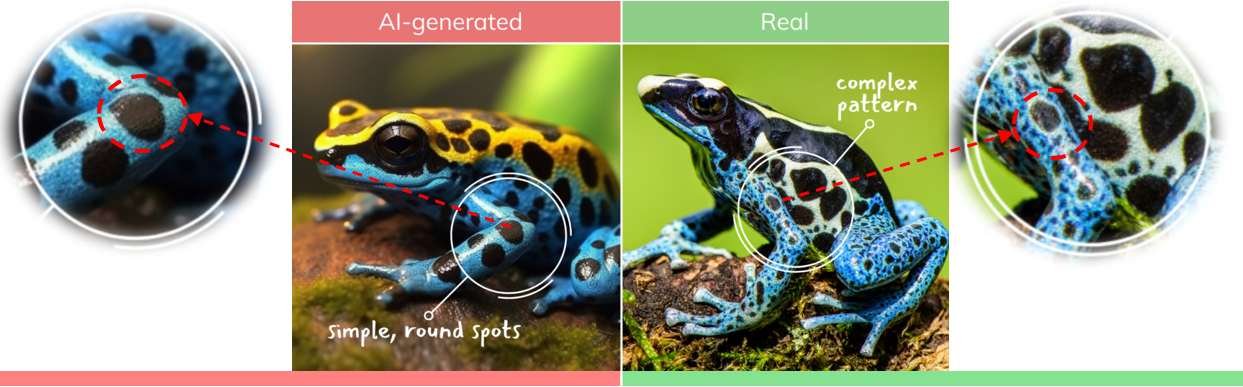
\includegraphics[width=0.9\linewidth]{ai-real-samples-1b.png}
		\begin{minipage}{0.9\linewidth}
			\caption{Ảnh tạo sinh \textit{(trái)} và ảnh thật \textit{(phải)}, được phân biệt dựa vào mức độ chi tiết trên hoa văn của đối tượng. \textit{Nguồn: \url{https://elearn.eb.com}}}
			\label{fig:ai-real-samples-1b}
		\end{minipage}
	\end{figure}\\
	%
	Bênh cạnh đó để huấn luyện mô hình \textit{"hiểu"} được các điểm bất hợp lý là bài toán khó, yêu cầu dữ liệu huấn luyện lớn và việc gán nhãn vị trí bất hợp lý trên hình ảnh cần nhiều chi phí, vì vậy hướng tiếp cận này ít được sử dụng hiện nay, tuy nhiên đây có thể là hướng phát triển tiềm năng khi kết hợp với mô hình ngôn ngữ lớn vì nó cho đưa ra được giải thích cho kết quả dự đoán.
	%
	\item Phát hiện hình ảnh giả mạo dựa vào phân tích, rút trích các đặc trưng tần số hay đặc trưng không gian trên hình ảnh. Hướng tiếp cận này mặc dù đem lại kết quả cao, ít phụ thuộc vào ngữ nghĩa của hình ảnh, tuy nhiên các kiến trúc mô hình khác nhau sẽ tạo ra những dấu vết khác nhau, do đó, thách thức lớn trong việc tìm ra đặt trưng chung và có hiệu quả trên nhiều mô hình tạo sinh (Hình~\ref{fig:gan-fingerprints-1}).
	
	\begin{figure}[htp]
		\centering
		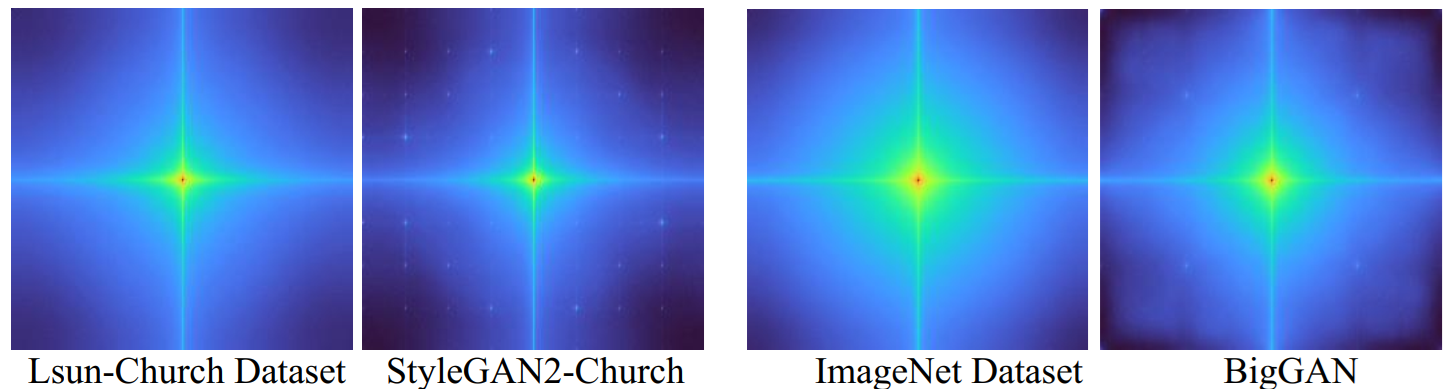
\includegraphics[width=1.0\textwidth]{gan-fingerprints-1.png}
	    \vspace{10pt} % Thay đổi khoảng cách giữa ảnh và chú thích
	    
		\begin{minipage}{\linewidth}
			\caption{Trung bình phổ Fourier của 2,000 hình ảnh từ tập dữ liệu Lsun \textit{(trái)} và ImageNet \textit{(phải)}, các dấu vết khác nhau giữa mô hình StyleGAN2 và BigGAN thể hiện ở hình 2 và 4 từ trái sang.}
			\label{fig:gan-fingerprints-1}
		\end{minipage}
	\end{figure}
	%
\end{itemize}
%
Ảnh tạo sinh rất đa dạng về nội dung, hình thức và được tạo ra theo trí tưởng tượng vô hạn của người dùng. Các hướng tiếp cận cho độ chính xác cao hiện nay, đều tận dụng sức mạnh của kỹ thuật học sâu. Tuy nhiên, dữ liệu dùng để huấn luyện các mô hình này không đủ đại diện cho toàn bộ ảnh giả mạo, cụ thể dữ liệu huấn luyện chỉ chứa một số lượng hữu hạn các đối tương trong thế giới thực, nhưng trong thực tế các đối tượng trong ảnh giả mạo có thể nằm ngoài tập huấn luyện, đây là một khó khăn cơ bản của bài toán này.

Khó khăn trong việc trả lời câu hỏi \textit{"mô hình đã dựa vào đâu để đưa ra kết luận?"}, đây là khó khăn chung của việc ứng dụng kỹ thuật học sâu, và trong nhiệm vụ phát hiện ảnh giả mạo thì yêu cầu tính \textit{"giải thích được"} càng quan trọng. Các đặc điểm thể hiện một hình ảnh là giả mạo thường không thể nhận biết một cách trực quan mà là qua sự tổng hợp rút trích đặc trưng của mạng học sâu, do tính chất phức tạp của các mô hình này, việc cung cấp giải thích rõ ràng và minh bạch cho các quyết định của mô hình là một thách thức lớn.

\section{Đóng góp của luận văn}
Luận văn có những đóng góp cơ bản sau:
\begin{itemize}
	\item Luận văn đã đề xuất một bộ lọc mới làm tăng độ chính xác, tăng tốc độ hội tụ trong quá trình huấn luyện mô hình, đồng thời phương pháp này yêu cầu kiến trúc mạng đơn giản hơn nhiều phương pháp khác nhưng vẫn cho độ chính xác cao.
	\item \textcolor{red}{Thực hiện 2 thử nghiệm mở rộng, cho thấy hiệu quả của phương pháp trên nhiều tập dữ liệu, nhiều mô hình tạo sinh khác nhau.}
	\item \textcolor{red}{Phương pháp được đề xuất có tiềm năng ứng dụng rộng hơn cho bài toán phân tích hình ảnh pháp y (phát hiện thao tác sao chép, chỉnh sửa...).}
\end{itemize}









